%%=============================================================================
%% Methodologie
%%=============================================================================

\chapter{\IfLanguageName{dutch}{Methodologie}{Methodology}}%
\label{ch:methodologie}

De methodologie van dit onderzoek is opgebouwd als een iteratief onderzoeks- en ontwikkeltraject dat in vier hoofdfasen wordt uitgevoerd. Elke fase levert een concreet deelresultaat op dat als input dient voor de volgende stap. Deze proefondervindelijke en experimentele aanpak is essentieel omdat het evalueren van machine learning-modellen voor AI-detectie een continu proces is van dataverzameling, preprocessing, modeltraining, robuustheidstesting en interpretatie. De gekozen methoden zijn sterk kwantitatief onderbouwd en sluiten aan bij de best practices uit actueel academisch onderzoek naar deepfake-detectie.

De gehele implementatie is uitgevoerd in \textbf{Python 3.10+} met behulp van \textit{PyTorch}, \textit{scikit-learn}, \textit{timm} (PyTorch Image Models) en \textit{Grad-CAM}. De trainingen zijn uitgevoerd op Google Colab met GPU-acceleratie (NVIDIA T4), met speciale aandacht voor hardwareoptimalisatie om out-of-memory crashes te voorkomen.

%% =============================================================================
%% FASE 1: DATASET OPBOUWEN & PRE-PROCESSING
%% =============================================================================

\section{Fase 1: Dataverzameling, Analyse en Pre-processing}
\label{sec:fase1}

In de eerste fase wordt de reikwijdte van de te detecteren AI-manipulaties afgebakend en wordt een fundamentele dataset opgebouwd. Dit is cruciaal omdat:
\begin{itemize}
    \item Bestaande modellen vaak falen op ongeziene data als zij niet adequaat zijn getraind
    \item Klasse-onbalans (meer echte dan valse foto's) kan de modeltraining ernstig verstoren
    \item Data-artefacten kunnen leiden tot valse patronen die het model leert in plaats van echte manipulatiesignalen
\end{itemize}

\subsection{Datasetselectie en Verdeling}

Voor dit onderzoek worden twee primaire datasets gebruikt:

\begin{enumerate}
    \item \textbf{DeepDetect-2025 Dataset:} Deze Kaggle-dataset (Ayushmandatta1/deepdetect-2025) bevat moderne AI-gegenereerde gezichten en authentieke foto's. Dit is de primaire trainings- en validatiedataset. De dataset is onderverdeeld in:
    \begin{itemize}
        \item \textbf{Trainingsset (70\%):} Gebruikt voor het optimaliseren van de modelgewichten
        \item \textbf{Validatieset (15\%):} Gebruikt voor hyperparameter-tuning en modelselectie
        \item \textbf{Testset (15\%):} Ongeziene data voor eindgebruikevaluatie
    \end{itemize}
    
    \item \textbf{140k Real and Fake Faces Dataset (xhlulu/140k-real-and-fake-faces):} Dit is de \textbf{ultieme robuustheidstest}. Dit dataset wordt \textit{niet} gebruikt voor training, maar uitsluitend voor cross-dataset evaluatie. Dit simuleert de echte wereld waar een deepfake-detectie-systeem moet omgaan met data uit volledig andere bronnen dan waarop het is getraind.
\end{enumerate}

Deze tweeledige aanpak volgt het \textit{generalisatie-paradoxon}: een model met perfecte prestaties op de trainingsdata kan volledig falen op nieuwe data. Door beide datasets te gebruiken, kunnen we beide gebreken meten.

\subsection{Dataset-statistieken en Visuele Inspectie}

Voordat training plaatsvindt, zijn uitgebreide analysefuncties toegepast om de dataset-karakteristieken te begrijpen. De volgende parameters zijn gemeten:

\inputminted[fontsize=\footnotesize, linenos, frame=lines]{python}{code/dataset_analysis.py}

%Figuur \ref{fig:dataset_distribution} toont de klasse-verdeling van de DeepDetect-2025 trainingsset. Dit visualiseert eventuele klasse-onbalans, die gecorrigeerd moet worden via \textit{WeightedRandomSampler} in PyTorch.
\begin{figure}[H]
    \centering
    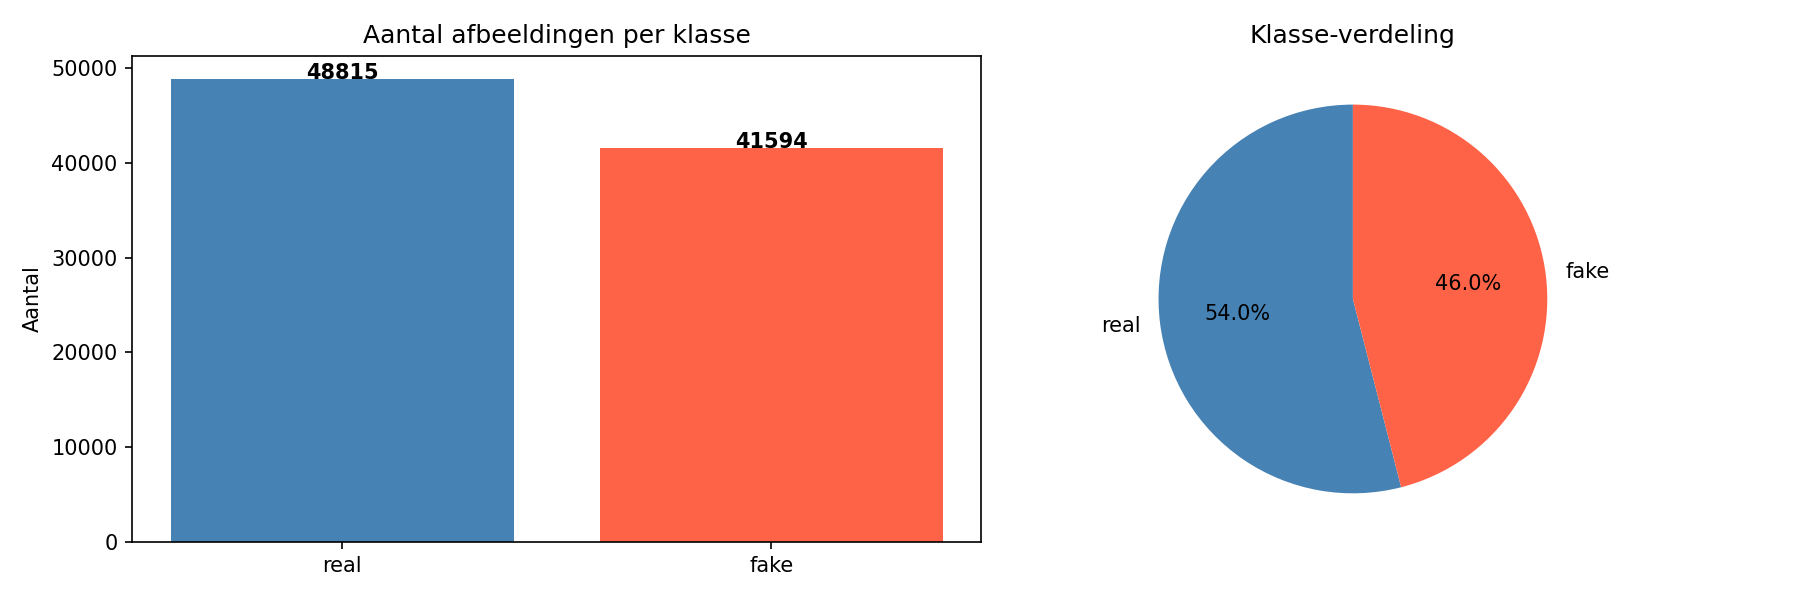
\includegraphics[width=0.9\textwidth]{../ipynb_output/ViT_results/dataset_distribution.png}
    \centerline{\small (a) DeepDetect-2025}
    \caption[Verdeling van de dataset]{Barchart en piechart van de klasse-verdeling, dit visualiseert eventuele klasse-onbalans.}
\end{figure}
% TODO: Genereer en voeg figuur in: dataset_distribution.png (class distribution bar chart)

\subsection{Klasse-onbalans en Balanceringsmechanismen}

In praktische datasets is klasse-onbalans een veelvoorkomend probleem. Als bijvoorbeeld 70\% van de afbeeldingen echt is en 30\% nep, kan een model bereikt worden met 70\% accuraatheid door alles als "echt" te voorspellen. Dit wordt voorkomen door:

\begin{enumerate}
    \item \textbf{WeightedRandomSampler:} Geeft hogere bemonsteringskansen aan de minderheidsklasse (nep-foto's), zodat de model beide klassen gelijkmatig ziet.
    \item \textbf{Class Weighting in Loss Function:} De verliesfunctie krijgt gewichten die inversely proportioneel zijn aan de klassefrequentie.
\end{enumerate}

%\inputminted[fontsize=\footnotesize, linenos, frame=lines]{python}{code/class_weighting.py}

\subsection{Data Pre-processing en Augmentatie Pipeline}

Voordat afbeeldingen de neurale netwerken bereiken, ondergaan zij een gestandaardiseerde pre-processing pijplijn:

\begin{enumerate}
    \item \textbf{Resize naar 224×224 pixels:} De standaard voor ImageNet-voorgetrainde modellen. Dit balanceert computationele efficiëntie met informatiebehoud.
    
    \item \textbf{ImageNet-normalisatie:} Tensor-waarden worden genormaliseerd met de ImageNet MEAN en STD:
    $$\text{Tensor}_{\text{norm}} = \frac{\text{Tensor} - [0.485, 0.456, 0.406]}{[0.229, 0.224, 0.225]}$$
    Dit is essentieel omdat voorgetrainde modellen worden geïnitialiseerd met weights die optimaal zijn voor ImageNet-genormaliseerde inputs.
    
    \item \textbf{Data Augmentatie voor Training:} Op de trainingsset worden transformaties toegepast om overfitting te voorkomen:
    \begin{itemize}
        \item \textbf{Random Crop:} Simuleer verschillende snijhoeken
        \item \textbf{Random Horizontal/Vertical Flip:} Gezichten zijn niet altijd in dezelfde oriëntatie
        \item \textbf{Color Jitter:} Helderheid, contrast, verzadiging variëren
        \item \textbf{Random Erasing:} Simuleer occlusie (bijvoorbeeld een deel van het gezicht is verborgen)
        \item \textbf{Gaussian Blur:} Simuleer beperkte scherpte van sociale media
    \end{itemize}
    
    \item \textbf{Geen augmentatie voor Validatie/Test:} Deze sets gebruiken alleen resize + normalisatie voor objectieve evaluatie.
\end{enumerate}

\inputminted[fontsize=\footnotesize, linenos, frame=lines]{python}{code/transforms.py}

\subsection{Hardware-optimalisatie: Oplossing voor Out-of-Memory Crashes}

Tijdens implementatie op Google Colab ontstonden kritieke out-of-memory (OOM) crashes bij het parallel inladen van tienduizenden afbeeldingen. De root cause was het gebruik van \texttt{num\_workers > 0}, wat sub-processen spawnt die elk volledige batches in het RAM bufferen.

De oplossing:
\inputminted[fontsize=\footnotesize, linenos, frame=lines]{python}{code/dataloader_fix.py}

Dit toont het belang van het afstemmen van software-architectuur op beschikbare hardware-resources.

%% =============================================================================
%% FASE 2: MODELSELECTIE, TRAINING & EVALUATIE
%% =============================================================================

\section{Fase 2: Modelarchitectuur, Training en Evaluatie}
\label{sec:fase2}

In deze fase worden drie verschillende neurale netwerkarchitecturen geselecteerd, getraind en geëvalueerd. Elke architectuur heeft een unieke benadering voor patroonherkenning:

\subsection{Modelarchitecturen}

\begin{enumerate}
    \item \textbf{CNN (EfficientNet-B3):} 
    Convolutional Neural Networks excelleren in het detecteren van \textit{lokale} artefacten. Ze scannen het beeld met kleine convolutionele filters (3×3 of 5×5) om pixel-inconsistenties op te sporen, zoals:
    \begin{itemize}
        \item Randartefacten bij face-swap detectie
        \item Ruis-patronen van GAN-modellen
        \item Textuur-discontinuïteiten
    \end{itemize}
    EfficientNet-B3 is gekozen omdat het een goed evenwicht biedt tussen accuraatheid en computationele efficiëntie.
    
    \item \textbf{Vision Transformer (ViT-Base/16):}
    Vision Transformers verdelen het beeld in kleine "patches" (16×16 pixels) en gebruiken self-attention om relaties tussen alle patches simultaan te leren. Dit is krachtig voor \textit{globale} patronen, zoals:
    \begin{itemize}
        \item Asymmetrische belichting (ogen hebben verschillende helderheid)
        \item Inconsistentie in gezichtsgeometrie
        \item Globale kleurverschillen
    \end{itemize}
    ViT's zijn inherent beter in het capteren van langetermijn-afhankelijkheden.
    
    \item \textbf{Hybride Model (ConvNeXt-Small):}
    ConvNeXt is een moderne architectuur die de voordelen van CNN's (inductive bias, efficiëntie) combineert met transformer-concepten (skip connections, normalisatie). Dit zorgt voor een evenwicht tussen lokale detail-detectie en globale context-begrip.
\end{enumerate}

\subsection{Model Constructie}

De drie modellen worden dynamisch opgebouwd via een factory-functie, waarbij de pretrained ImageNet-gewichten worden geladen en de laatste classificatielaag wordt vervangen voor binaire classificatie (real vs. fake):

\inputminted[fontsize=\footnotesize, linenos, frame=lines]{python}{code/build_model.py}

Tabel \ref{tab:model_comparison} geeft een samenvatting van de modelparameters. Opgemerkt wordt dat ViT significant meer parameters heeft (86M vs. 12M voor CNN), wat impliceert dat ViT gevoeliger kan zijn voor overfitting op kleine datasets.

\begin{table}[h]
\centering
\caption{Vergelijking van modelarchitecturen}
\label{tab:model_comparison}
\begin{tabular}{l|r|r|r}
\textbf{Model} & \textbf{Architect.} & \textbf{Param.} & \textbf{Specialisatie} \\
\hline
CNN & EfficientNet-B3 & 12M & Lokale artefacten \\
ViT & ViT-Base/16 & 86M & Globale context \\
Hybride & ConvNeXt-Small & 50M & Lokaal + globaal \\
\end{tabular}
\end{table}

\subsection{Trainingssetup en Hyperparameters}

De training is uitgevoerd met de volgende geoptimaliseerde hyperparameters:

\begin{table}[h]
\centering
\caption{Trainings-hyperparameters}
\label{tab:hyperparams}
\begin{tabular}{l|l}
\textbf{Parameter} & \textbf{Waarde} \\
\hline
Batch Size & 32 \\
Learning Rate (initial) & $1 \times 10^{-4}$ \\
Optimizer & AdamW \\
Weight Decay & $1 \times 10^{-4}$ \\
Loss Function & CrossEntropyLoss \\
Scheduler & Cosine Annealing \\
Max Epochs & 30 \\
Gradient Clip & 1.0 (max norm) \\
\end{tabular}
\end{table}

\textbf{Motivatie van keuzes:}

\begin{itemize}
    \item \textbf{AdamW:} Geavanceerde optimizer met gewichtsverzwakking, beter dan standaard Adam voor deep learning.
    \item \textbf{Cosine Annealing:} Learning rate daalt geleidelijk volgens een cosinuscurve. Dit helpt om betere lokale minima te bereiken.
    \item \textbf{Gradient Clipping:} Voorkomt "exploding gradients" die training kunnen destabiliseren.
    \item \textbf{Cross-Entropy Loss:} Standaard voor multi-class classificatie met logits-output.
\end{itemize}

\inputminted[fontsize=\footnotesize, linenos, frame=lines]{python}{code/training_loop.py}

%Figuur \ref{fig:training_curves} toont de training-curves voor alle drie modellen. Deze visualisaties zijn essentieel voor het detecteren van overfitting (wanneer val_loss stijgt terwijl train_loss daalt) of underfitting.
\begin{figure}[H]
    \centering
    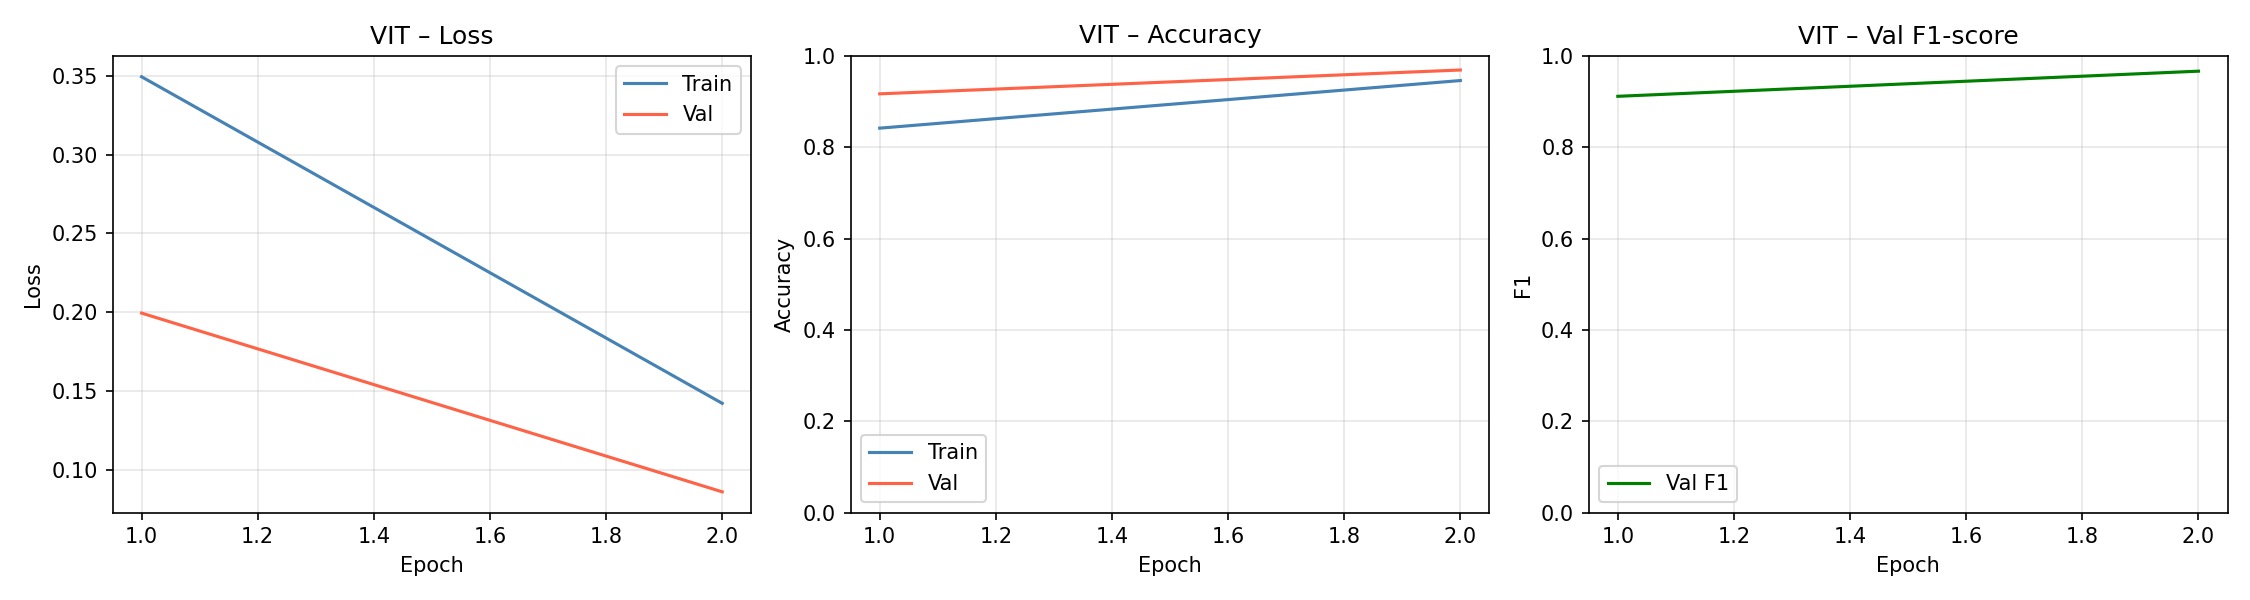
\includegraphics[width=0.9\textwidth]{../ipynb_output/ViT_results/training_curves.png}
    \centerline{\small (a) Training Curves voor ViT-Base/16 op DeepDetect-2025}
    
    \vspace{1cm}
    
    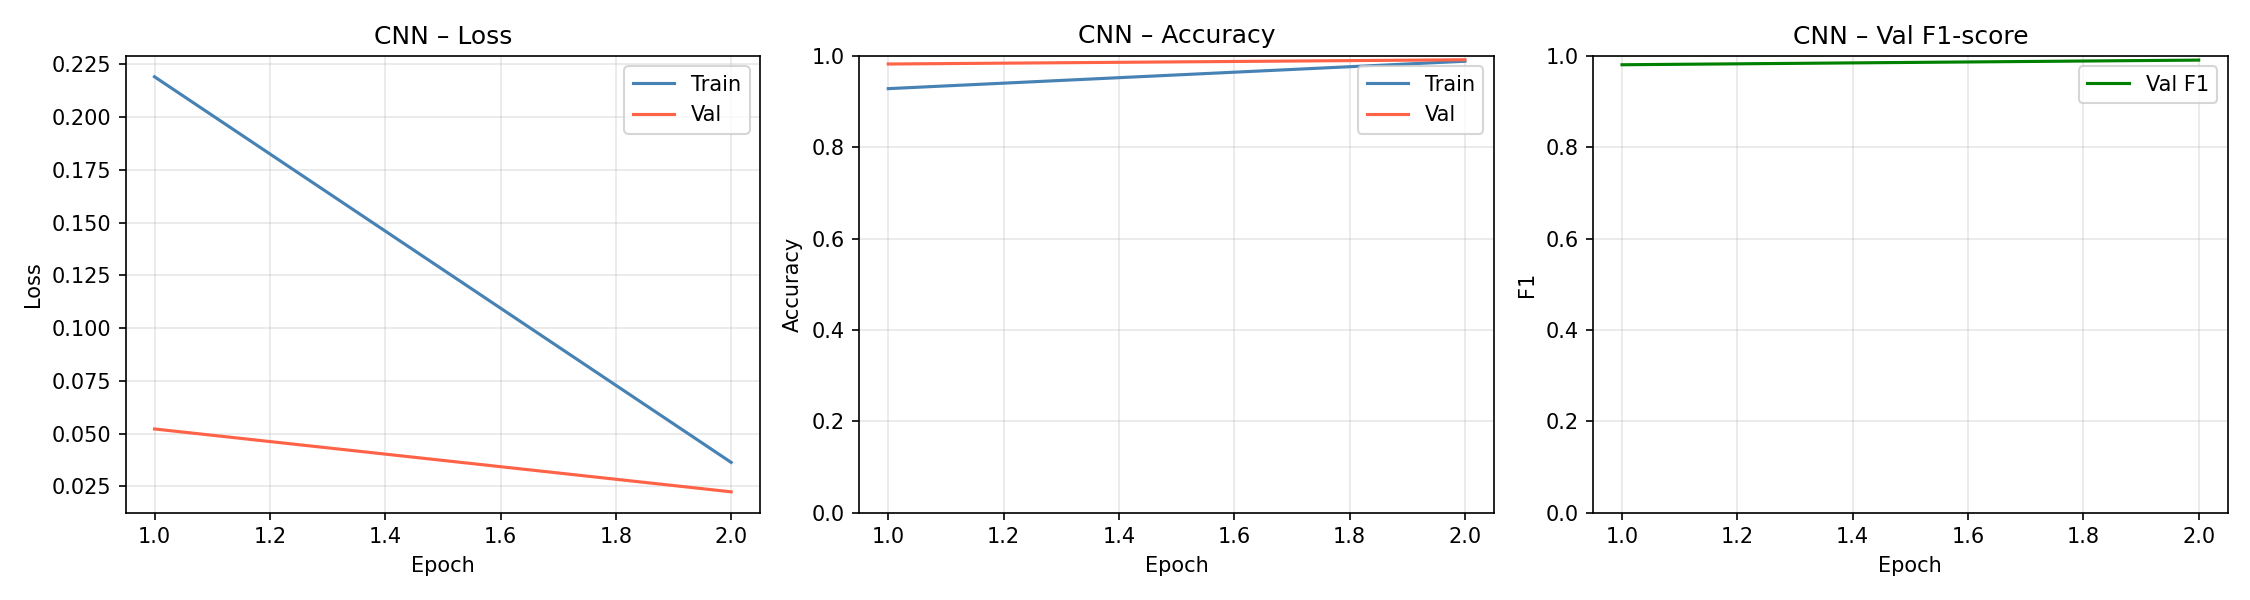
\includegraphics[width=0.9\textwidth]{../ipynb_output/CNN_results/training_curves.png}
    \centerline{\small (b) Training Curves voor CNN op DeepDetect-2025}

    \vspace{1cm}
    
    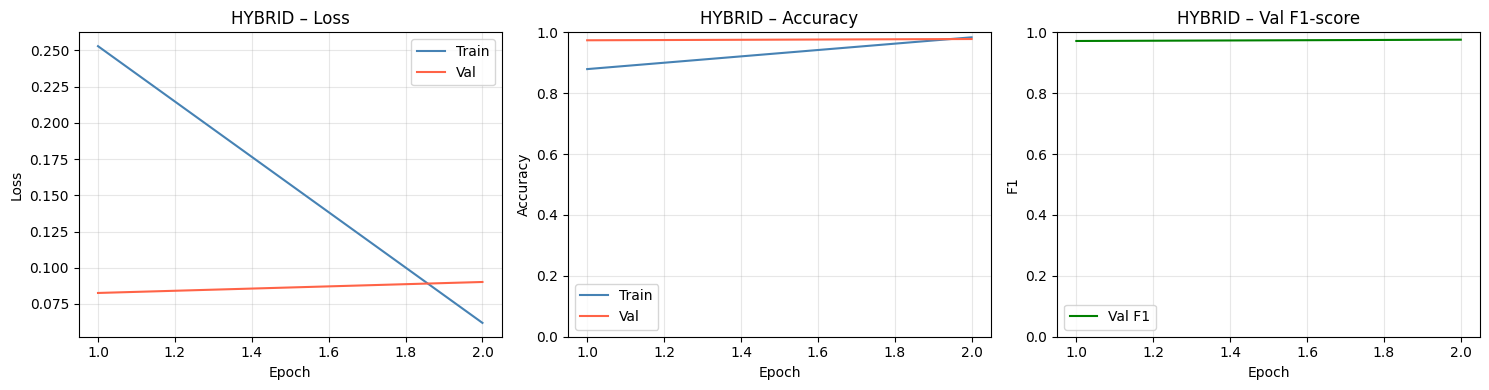
\includegraphics[width=0.9\textwidth]{../ipynb_output/Hybrid_results/training_curves.png}
    \centerline{\small (c) Training Curves voor Hybride model op DeepDetect-2025}
    
    \caption[Training Curves op DeepDetect-2025]{Training Curves voor de DeepDetect-2025 dataset. Deze figuren tonen hoe elk model presteert.}
\end{figure}
% TODO: Genereer en voeg figuur in: training_curves.png (train/val loss en accuracy per epoch)

\subsection{Evaluatiemetrieken en Wiskundige Verantwoording}

De evaluatie van de modellen vereist meer dan enkel \textit{accuracy}. In de context van deepfake-detectie kan een vals-positief resultaat (een authentieke foto labelen als nep) leiden tot onterechte beschuldigingen of censuur. Een diepgaande wiskundige analyse is daarom noodzakelijk.

De basis van alle metrieken is de \textbf{Confusion Matrix}, opgebouwd uit vier componenten:

\begin{table}[h]
\centering
\caption{Confusion Matrix voor binaire classificatie}
\label{tab:confusion_matrix}
\begin{tabular}{c|c|c}
& \textbf{Voorspeld: Real} & \textbf{Voorspeld: Fake} \\
\hline
\textbf{Echt: Real} & TN (True Negative) & FP (False Positive) \\
\textbf{Echt: Fake} & FN (False Negative) & TP (True Positive) \\
\end{tabular}
\end{table}

\textbf{Afgeleid metrieken:}

\begin{enumerate}
    \item \textbf{Accuracy:} Algemeen percentage correct geclassificeerd
    $$\text{Accuracy} = \frac{TP + TN}{TP + TN + FP + FN}$$
    \textit{Waarschuwing:} Accuracy verbergt klassespecifieke prestaties en kan misleidend zijn bij klasse-onbalans.
    
    \item \textbf{Precision (Precisie):} Van alle foto's die het model als "FAKE" labelt, hoeveel waren daadwerkelijk nep?
    $$\text{Precision} = \frac{TP}{TP + FP}$$
    Dit is kritisch: een lage precision betekent veel onterechte beschuldigingen.
    
    \item \textbf{Recall (Gevoeligheid):} Van alle werkelijk neppe foto's, hoeveel herkende het model?
    $$\text{Recall} = \frac{TP}{TP + FN}$$
    Dit meet: \textit{miste het model veel manipulaties?}
    
    \item \textbf{F1-Score:} Harmonische gemiddelde van Precision en Recall. Dit is de \textbf{leidende metriek} in dit onderzoek:
    $$F1 = 2 \cdot \frac{\text{Precision} \cdot \text{Recall}}{\text{Precision} + \text{Recall}}$$
    
    F1 is robuuster dan accuracy, vooral bij klasse-onbalans. Het balanceert beide fouttypes.
    
    \item \textbf{ROC-AUC (Area Under the ROC Curve):} Plot True Positive Rate vs. False Positive Rate op alle mogelijke drempelwaarden:
    $$\text{ROC-AUC} = \int_0^1 \text{TPR}(t) \, d(\text{FPR}(t))$$
    AUC geeft aan hoe goed het model de twee klassen scheidt, onafhankelijk van de drempel.
    
    \item \textbf{Average Precision (AP) / PR-AUC:} Integreert de Precision-Recall curve. Dit is **nog belangrijker dan ROC-AUC** voor ongebalanceerde datasets omdat het meer gewicht geeft aan precision (vermijding van false positives):
    $$\text{AP} = \int_0^1 \text{Precision}(t) \, d(\text{Recall}(t))$$
\end{enumerate}

\subsubsection{Waarom Precision-Recall boven ROC voor deepfake-detectie?}

De ROC-curve is symmetrisch t.o.v. beide klassen: het weegt false positives en true positives gelijk. Voor deepfake-detectie is dit suboptimaal omdat:

\begin{itemize}
    \item Een \textbf{false positive} (authentieke foto als fake) kan mensenrechten schenden (censuur, haatcampagnes)
    \item Een \textbf{false negative} (fake niet gedetecteerd) kan desinformatie verspreiden, wat minder direct schadelijk is
\end{itemize}

De PR-curve weegt false positives zwaarder, wat beter aansluit bij de praktische behoeften van het systeem.

\inputminted[fontsize=\footnotesize, linenos, frame=lines]{python}{code/eval_function.py}

%Figuur \ref{fig:confusion_matrices} toont de confusion matrices voor DeepDetect-2025 en de 140k Real and Fake Faces dataset. Figuur \ref{fig:roc_pr_curves} toont de ROC- en PR-curves.
\begin{figure}[H]
    \centering
    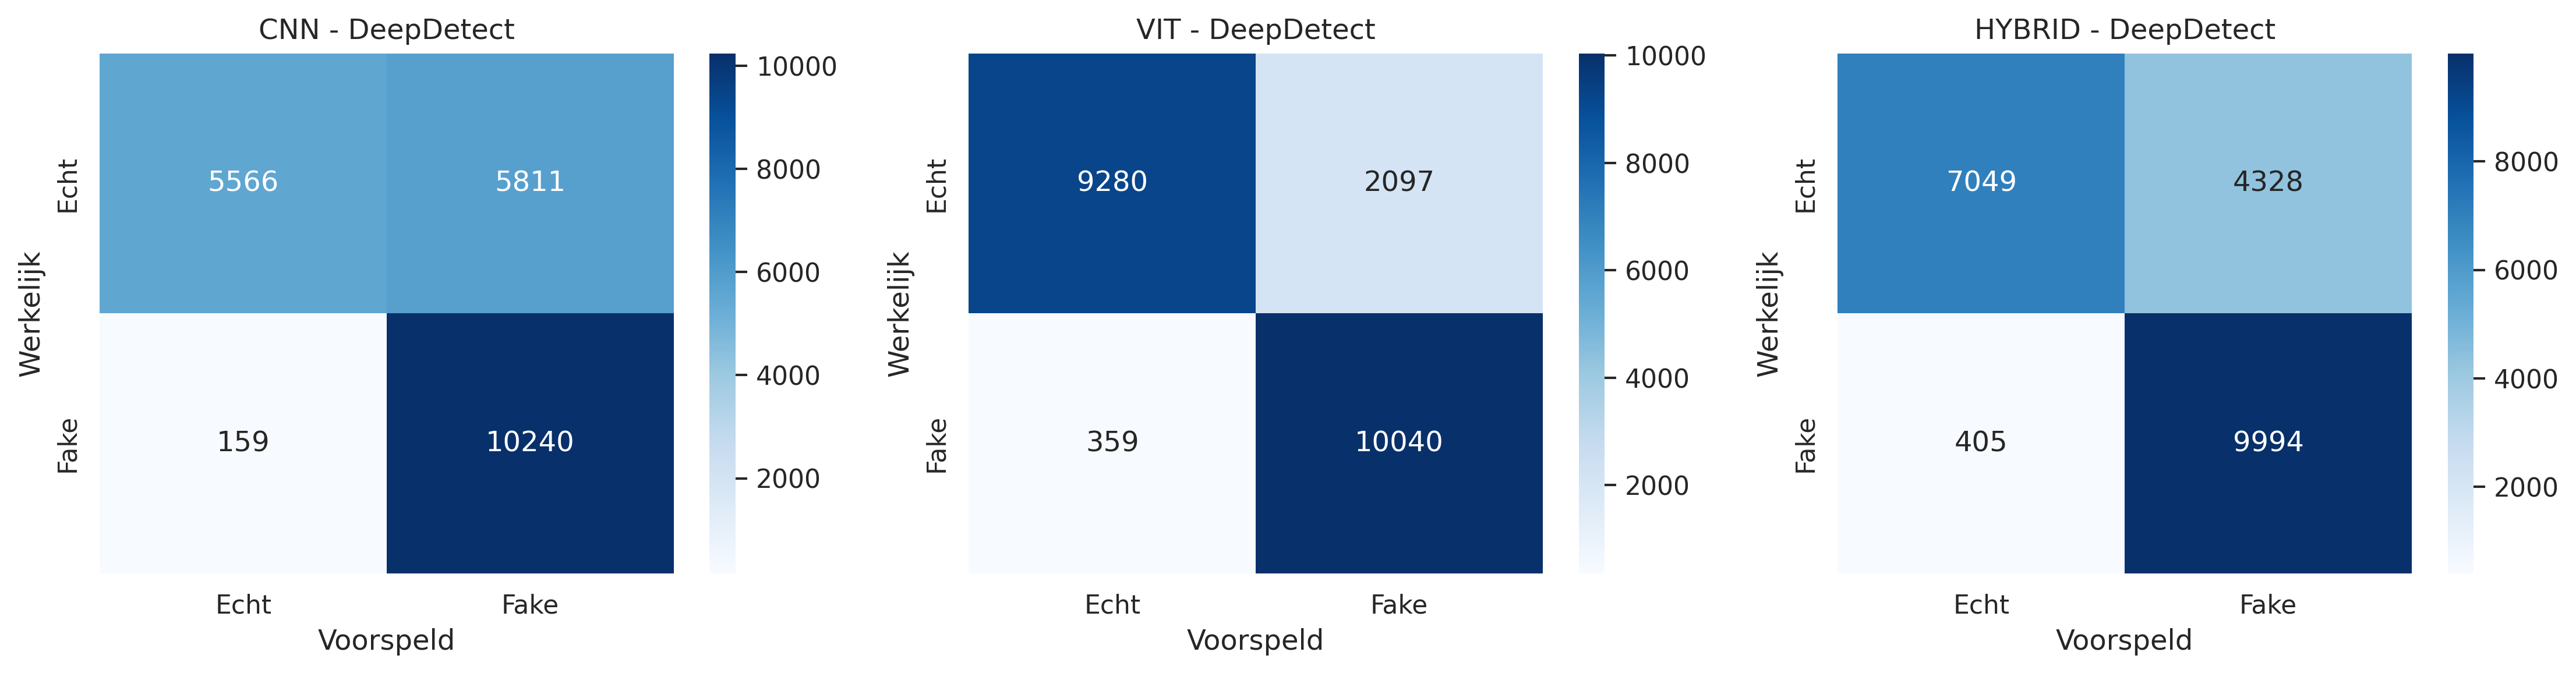
\includegraphics[width=0.9\textwidth]{../ipynb_output/confusion_matrices/CM_DeepDetect.png}
    \centerline{\small (a) DeepDetect-2025}
    
    \vspace{1cm}
    
    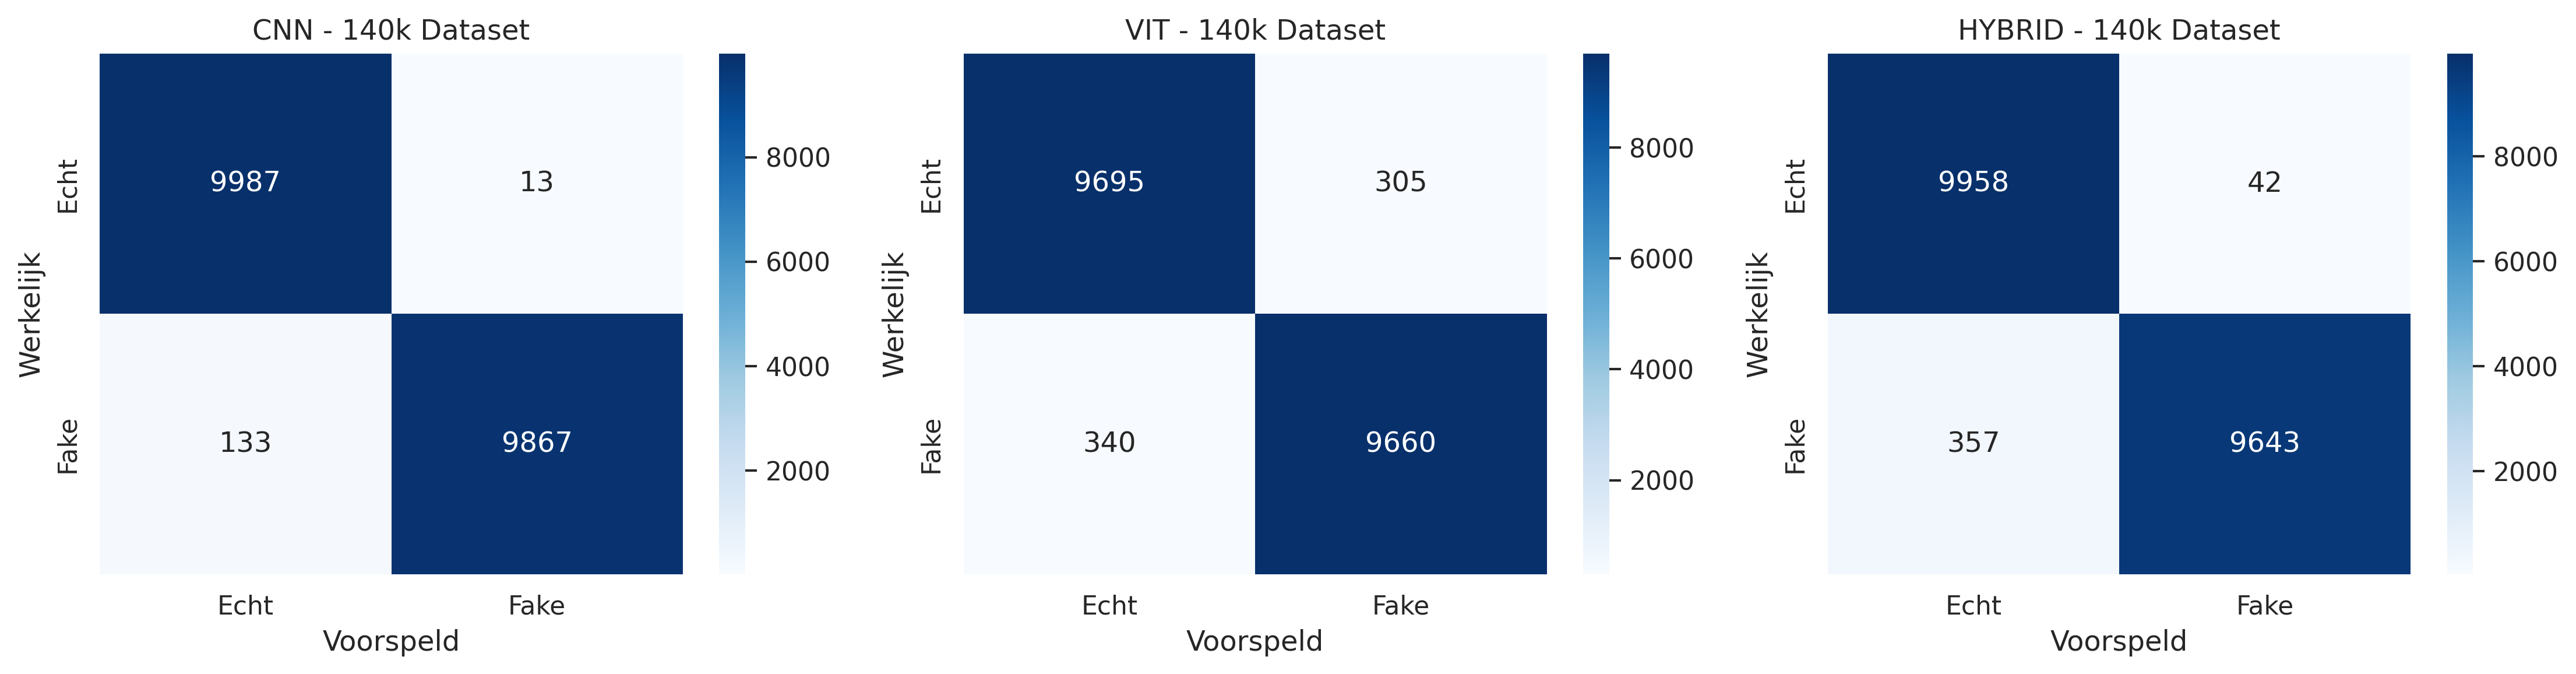
\includegraphics[width=0.9\textwidth]{../ipynb_output/confusion_matrices/CM_140k.png}
    \centerline{\small (b) 140k Real and Fake Faces}
    
    \caption[Confusion matrices voor DeepDetect-2025 en 140k.]{Confusion matrices voor de DeepDetect-2025 dataset en de 140k Real and Fake Faces dataset. Deze figuren tonen hoe het model per dataset echte en nepbeelden classificeert.}
\end{figure}
% TODO: Genereer en voeg figuren in:
% - confusion_matrices/CM_DeepDetect.png en confusion_matrices/CM_140k.png
% - roc_pr_curves.png (ROC en PR curves voor alle modellen)

%% =============================================================================
%% FASE 3: ROBUUSTHEIDSANALYSE & GENERALISATIE
%% =============================================================================

\section{Fase 3: Robuustheidsanalyse en Cross-Dataset Generalisatie}
\label{sec:fase3}

Modellen die hoog scoren in een laboratoriumomgeving presteren vaak aanzienlijk slechter wanneer ze worden geconfronteerd met real-world data. Afbeeldingen op sociale media worden gecomprimeerd, geschaald, gefilterd en bewerkt. Dit onderzoek implementeert een \textbf{tweeledige robuustheidsanalyse}:

\subsection{Synthetische Degradatie: JPEG-Compressie}

JPEG is het meest voorkomende beeldformaat op internet. Bij opslag gebruikt JPEG lossy-compressie: de afbeelding wordt opgeslagen in blokken van 8×8 pixels, en hoogfrequente details (vooral fijne textuur) worden verwijderd.

Onze hypothese: **CNN's (die sterk afhankelijk zijn van hoogfrequente ruis-patronen van GAN's) zullen sneller degraderen dan ViT's (die op globale patternherkenning focussen).**

\inputminted[fontsize=\footnotesize, linenos, frame=lines]{python}{code/jpeg_compression.py}

%Figuur \ref{fig:robustness_jpeg} toont de resultaten. Dit test niet alleen de modelprestaties, maar simuleert ook echte-wereld voorwaarden waarbij afbeeldingen meerdere keren gecomprimeerd worden.

% TODO: Genereer en voeg figuur in: robustness_jpeg.png (F1-score vs JPEG kwaliteit voor 3 modellen)

\subsection{De Ultieme Generalisatietest: Cross-Dataset Evaluatie}

De tweede en kritiekste robuustheidstest is evaluatie op de **volledig ongeziene 140k Real and Fake Faces dataset**. Deze dataset is niet gebruikt voor training of validatie. Dit simuleert scenario's waarbij het deepfake-detectiesysteem wordt ingezet op foto's van volkomen andere bronnen (andere camera's, apps, generatoren).

Dit is essentieel omdat:

\begin{enumerate}
    \item \textbf{Dataset Bias:} Modellen kunnen specifieke artefacten van de trainingsdata leren (achtergronden, belichting, gezichtskenmerken) in plaats van echte manipulatiesignalen.
    
    \item \textbf{Generalisatie:} Cross-dataset evaluatie meet of het model daadwerkelijk de \textit{semantiek} van AI-manipulaties heeft geleerd.
    
    \item \textbf{Praktische Bruikbaarheid:} Een model dat goed generalisert heeft daadwerkelijke waarde voor industriële toepassing.
\end{enumerate}

De 140k dataset wordt op identieke wijze geëvalueerd als de DeepDetect testset: dezelfde pre-processing, dezelfde modellen, dezelfde metrieken. Het is echter verboden om de resulaten te gebruiken voor hyperparameter-tuning; dit zou leiden tot "test data leakage."

%% =============================================================================
%% FASE 4: MODEL-INTERPRETATIE VIA GRAD-CAM
%% =============================================================================

\section{Fase 4: Explainable AI via Grad-CAM Heatmaps}
\label{sec:fase4}

Het "black-box" probleem van deep learning is fundamenteel: ook al geeft een model correcte voorspellingen, het is niet altijd duidelijk \textit{waarom}. Dit is problematisch voor deepfake-detectie, omdat:

\begin{itemize}
    \item \textbf{Auditing:} Regelgevers vereisen transparantie ("Waarom classificeerde het systeem deze foto als nep?")
    \item \textbf{Bias-detectie:} Zonder interpretatie kunnen we niet zien of het model discriminerende patronen leert.
    \item \textbf{Vertrouwen:} Gebruikers zijn voorzichtiger met systemen die hun beslissingen kunnen uitleggen.
\end{itemize}

De oplossing is \textbf{Explainable AI (XAI)}. Dit onderzoek implementeert **Grad-CAM++** (Gradient-weighted Class Activation Mapping++), een geavanceerde versie van Grad-CAM.

\subsection{Grad-CAM Theorie}

Grad-CAM berekent de belangrijkheid van pixels door te meten hoe sterk gradiënten (afgeleides) van de voorspelde klasse terugvloeien naar de feature maps:

$$\text{Importance}_{i,j} = \sum_k \underbrace{\frac{\partial y_{\text{fake}}}{\partial A^k_{i,j}}}_{\text{Gradient naar pixel}} \cdot \underbrace{A^k_{i,j}}_{\text{Activatie}}$$

Een hoge waarde betekent: **"Een kleine verandering in deze pixel zou grote verandering in de 'fake'-kans veroorzaken"** – dus het model focust erop.

Grad-CAM++ verbetert standaard Grad-CAM door multiple gradient-wegen te wegen, wat robuuster is tegen ruis.

\subsection{Implementatie en Fout-selectie}

\inputminted[fontsize=\footnotesize, linenos, frame=lines]{python}{code/gradcam_impl.py}

% TODO: Genereer en voeg figuren in:
% - gradcam_cnn.png (Grad-CAM++ heatmaps voor CNN)
% - gradcam_vit.png (Grad-CAM++ heatmaps voor ViT)
% - gradcam_hybrid.png (Grad-CAM++ heatmaps voor Hybrid)
% Voeg deze in met \begin{figure} en \includegraphics

\subsection{Fout-Analyse: Most Confident Errors}

Een belangrijk inzicht: niet alle fouten zijn gelijk. Een model dat 60\% zeker is van een fout is anders dan één die 99\% zeker is.

Dit onderzoek richt zich op **"most confident errors"** – fouten waarbij het model zeer hoog vertrouwen had. Dit zegt ons waar het model het hardst faalt:

\inputminted[fontsize=\footnotesize, linenos, frame=lines]{python}{code/confident_errors.py}

Dit biedt inzicht in welke soorten deepfakes het model mist, en kan gebruikt worden voor iteratieve modelverbetering.

\subsection{Threshold Optimization}

Standaard classifiers gebruiken een drempel van 0.5: als $P(\text{fake}) > 0.5$, voorspel "fake". Maar dit is niet altijd optimaal.

In deepfake-detectie kan een hogere drempel wenselijk zijn: liever 10 nep-foto's missen dan 1 echte foto onterecht beschuldigen (false positive).

\inputminted[fontsize=\footnotesize, linenos, frame=lines]{python}{code/threshold_optim.py}

%Figuur \ref{fig:threshold_analysis} toont deze analyse voor elk model.

% TODO: Genereer en voeg figuur in: threshold_analysis.png (F1-score vs threshold voor 3 modellen)

%% =============================================================================
%% SAMENVATTING METHODOLOGIE
%% =============================================================================

\section{Samenvatting Methodologische Aanpak}

Dit onderzoek volgt een rigoureus, iteratief proces:

\begin{enumerate}
    \item \textbf{Fase 1:} Dataset-analyse, balancering, pre-processing, augmentatie
    \item \textbf{Fase 2:} Drie architecturen selecteren, trainen met geoptimaliseerde hyperparameters, uitgebreide evaluatie
    \item \textbf{Fase 3:} Robuustheid testen onder JPEG-compressie en ongeziene datasets
    \item \textbf{Fase 4:} Interpretatie via Grad-CAM, fout-analyse, drempel-optimalisatie
\end{enumerate}

Dit leidt tot een compleet plaatje: niet alleen \textit{hoe goed} de modellen presteren, maar ook \textit{waarom}, \textit{waar} ze falen, en \textit{hoe} ze in praktijk inzetbaar zijn.

% TODO CHECKLIST:
% [ ] Alle figuren gegenereerd en opgeslagen in OUTPUT_DIR/figures/
% [ ] Cross-dataset evaluatie uitgevoerd op 140k dataset
% [ ] Resultaten van robustness_jpeg() in figures/robustness_jpeg.png
% [ ] Grad-CAM heatmaps in figures/gradcam_*.png
% [ ] Threshold optimization plot in figures/threshold_analysis.png
% [ ] Training curves in figures/training_curves.png
% [ ] Confusion matrices in figures/confusion_matrices.png
% [ ] ROC/PR curves in figures/roc_pr_curves.png
% [ ] Dataset distribution in figures/dataset_distribution.png
% [ ] LaTeX compilatie met: pdflatex -shell-escape VandenabeeleMirkoBP.tex